\chapter{Results}\label{Ch:results}




In this section we will cover the main classification results, as well as some results that were obtained by looking at a subset of artifacts.
\section{Performance of CNN}
Even though CNNs are widely used for computer vision and object detection, we did not find them to be useful for artifact detection. The performance of CNN on three artifacts in in Table \ref{tab:cnn}. The reason we are not showing other artifacts in this table is that the CNN was not able to train on those artifacts (the loss function either got stuck in a local minimum or never converged). It must be noted that we did not spend much time on hyper parameter tuning, therefore better results could be reached by using other hyper parameters.

\begin{table}[h]
    \centering
    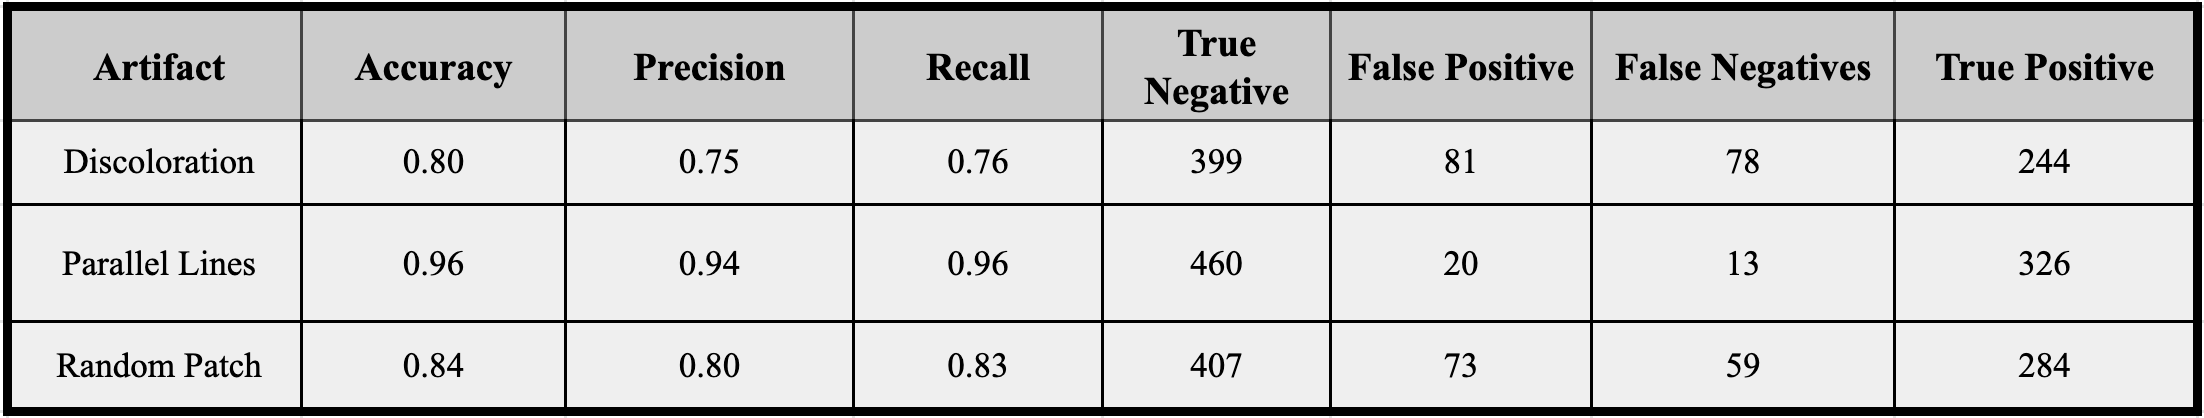
\includegraphics[scale=0.4]{images/CNN.png}
    \caption{Performance of Convolutional Neural Network  on Three Artifacts.}
    \label{tab:cnn}
\end{table}

\section{Performance of the ensemble on familiar games}
In training stage 1 and training stage 2, 25\% of the data (from data set A and data set B, respectively) was held out as test set. This means that when evaluating the models on these test sets, 1. the individual models have already seen the games in test set taken from data set A, and 2. the logistic regression has already seen (other images from) the games that were used in the test set taken from data set B. Table \ref{tab:models} and Figure \ref{fig:stage1} show the results of testing the individual models (after training stage 1). At this stage, the models are performing on familiar games. That is, the models have seen different images from the same games during training.\\

\noindent
As for the logistic regression, Table \ref{tab:stage2} contains the results of training the logistic regression (training stage 2 trained on data set B). We set aside 25\% of the data set B to test the performance of logistic regression on familiar games which turned out to have an accuracy of 84\%.
\begin{table}[h]
    \centering
    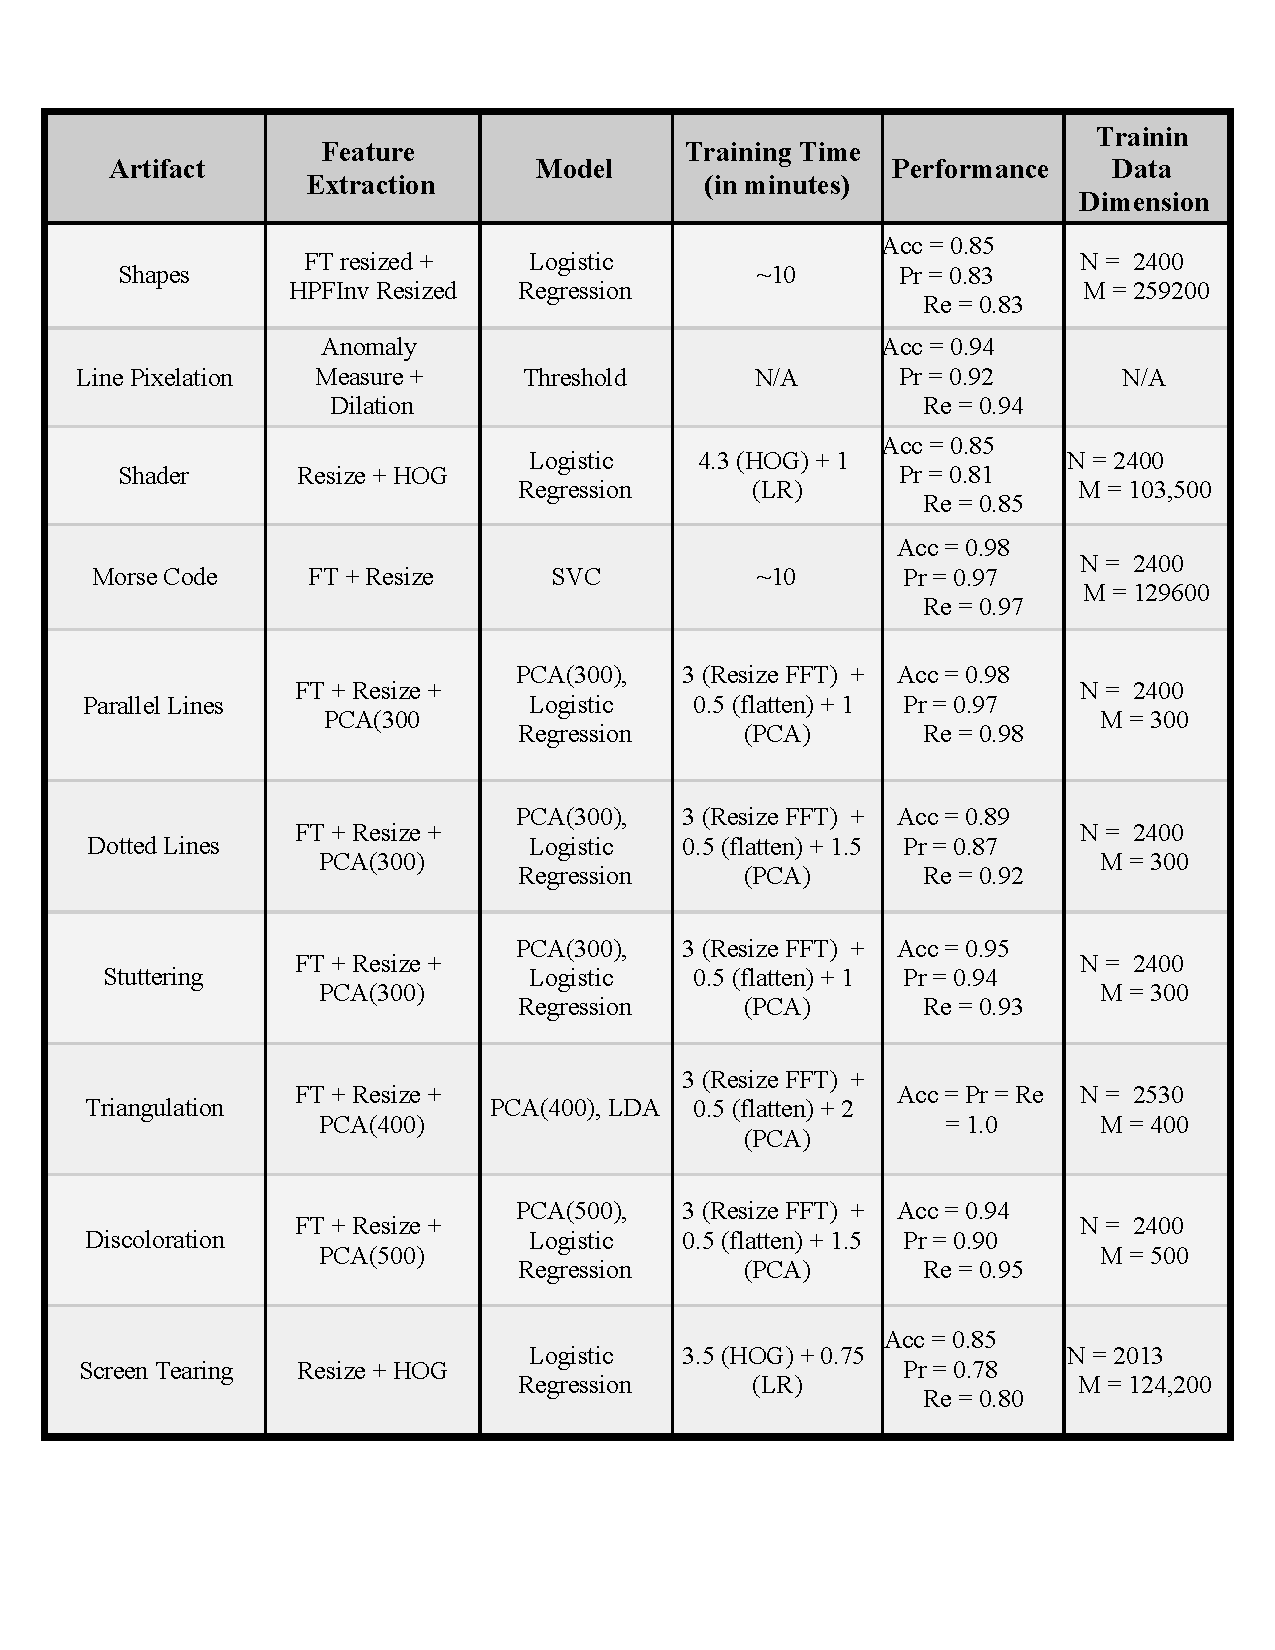
\includegraphics[scale=0.8]{tables/models.pdf}
    \caption{Performance of models in training stage 1.}
    \label{tab:models}
\end{table}

%\begin{landscape}
%\centering
%\begin{table}
%    \centering
%    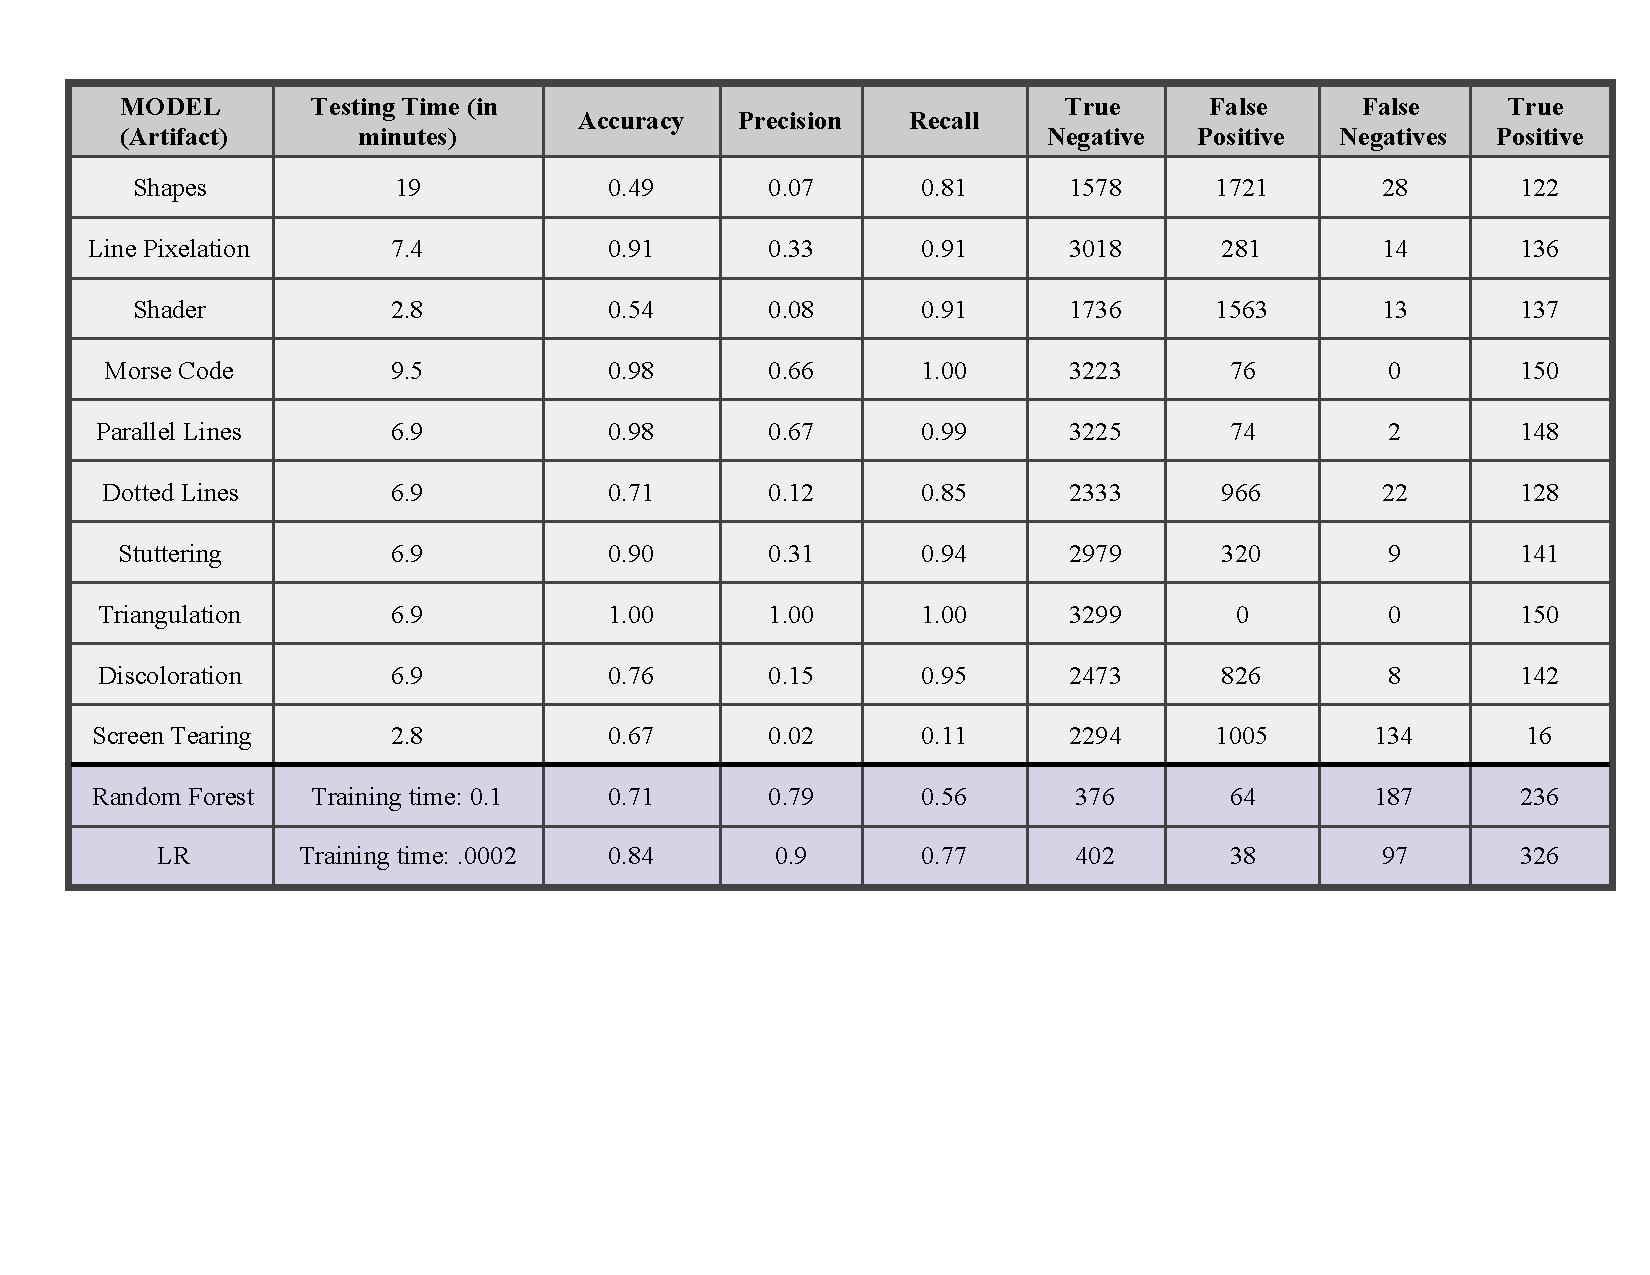
\includegraphics[scale=0.8]{tables/stage2.pdf}\\[-15ex]
%    \caption{Performance of models in training stage 2.}
%    \label{tab:stage2}
%\end{table}
%\end{landscape}

\begin{table}
\centering
\begin{tabular}{@{}lllll@{}}
\toprule
Model (Artifact) & Testing Time (min) & Accuracy & Precision & Recall  \\ \midrule
Shapes & 19 & 0.49 & 0.07 & 0.81\\
Line pixelation & 7.4 & 0.91 & 0.33 & 0.91\\
Shader & 2.8 & 0.54 & 0.08 & 0.91\\
Morse code & 9.5 & 0.98 & 0.66 & 1.00\\
Parallel lines & 6.9 & 0.98 & 0.67 & 0.99\\
Dotted line & 6.9 & 0.71 & 0.12 & 0.85\\
Stuttering & 6.9 & 0.90 & 0.31 & 0.94\\
Triangulation & 6.9 & 1.00 & 1.00 & 1.00\\
Discoloration & 6.9 & 0.76 & 0.15 & 0.95\\
Screen tearing & 2.8 & 0.67 & 0.02 & 0.11\\
\midrule
\bf{Random Forest} & \bf{N/A} & \bf{0.71} & \bf{0.79} & \bf{0.56}\\
\bf{Logistic Regression} & \bf{N/A} & \bf{0.84} & \bf{0.9} & \bf{0.77}\\\bottomrule
\end{tabular}
\caption{Performance of models after training stage 2.}
\label{tab:stage2}
\end{table}

\section{Performance of the ensemble on new games}
\noindent An important metric in assessing artifact detection models is generalizability. In our case, generalizability refers to the ability of the model to perform equally well when images come from games unseen during training. We can measure not only the generalizability of the final logistic regression, but also that of individual models. \\

\noindent
Recall that in training stage 2, even though the logistic regression has seen the games in dataset B, the individual models have not. Therefore the performance of the individual models in Table \ref{tab:stage2} is a measure of their generalizability to new games. Figure \ref{fig:stage2} is a visualization of the models in Table \ref{tab:stage2}. \\
 
\noindent
We also tested the generalizability of the ensemble model. For this purpose, we tested it on data set $C$ which it has never seen before, and obtained an accuracy of 69\%. The second row of \ref{tab:variation} contains other metrics on the performance of the logistic regression on the heldout test set. The performance metrics of the individual models on this test set is restricted to True Negative and False Positive (Table \ref{tab:test_models}). This is because our test data was labeled as 0 or 1, and therefore we cannot tell how many false negatives and true positives of a given model are the specific artifact type of the model, or other artifacts. \\

%maybe this should go to the Discussion chapter
\noindent The difference in performance of models in Table \ref{tab:models}
and Table \ref{tab:stage2} is that in Table \ref{tab:models}, not only are the individual models tested on games that they have seen before, but also they are tested on a dataset that only consists of normal images and the corrupted images that each model is trained to detect. In Table \ref{tab:stage2} the models are tested on images coming from games that they have never seen, in addition to corruptions they have never seen. In Table \ref{tab:stage2} we can see that the Shapes and Shader models have low accuracy of 0.49 and 0.54 respectively. Therefore we conduct an experiment where we excluded these two models while keeping the artifacts in the data (Table \ref{tab:variation}). Additionally we retrained the logistic regression after excluding the screen tearing model and artifact from the data. We also trained the logistic regression on probability outputs instead of binary outputs. The results are shown in Table \ref{tab:variation} and Figure \ref{fig:probability}.


\begin{figure}
    \centering
    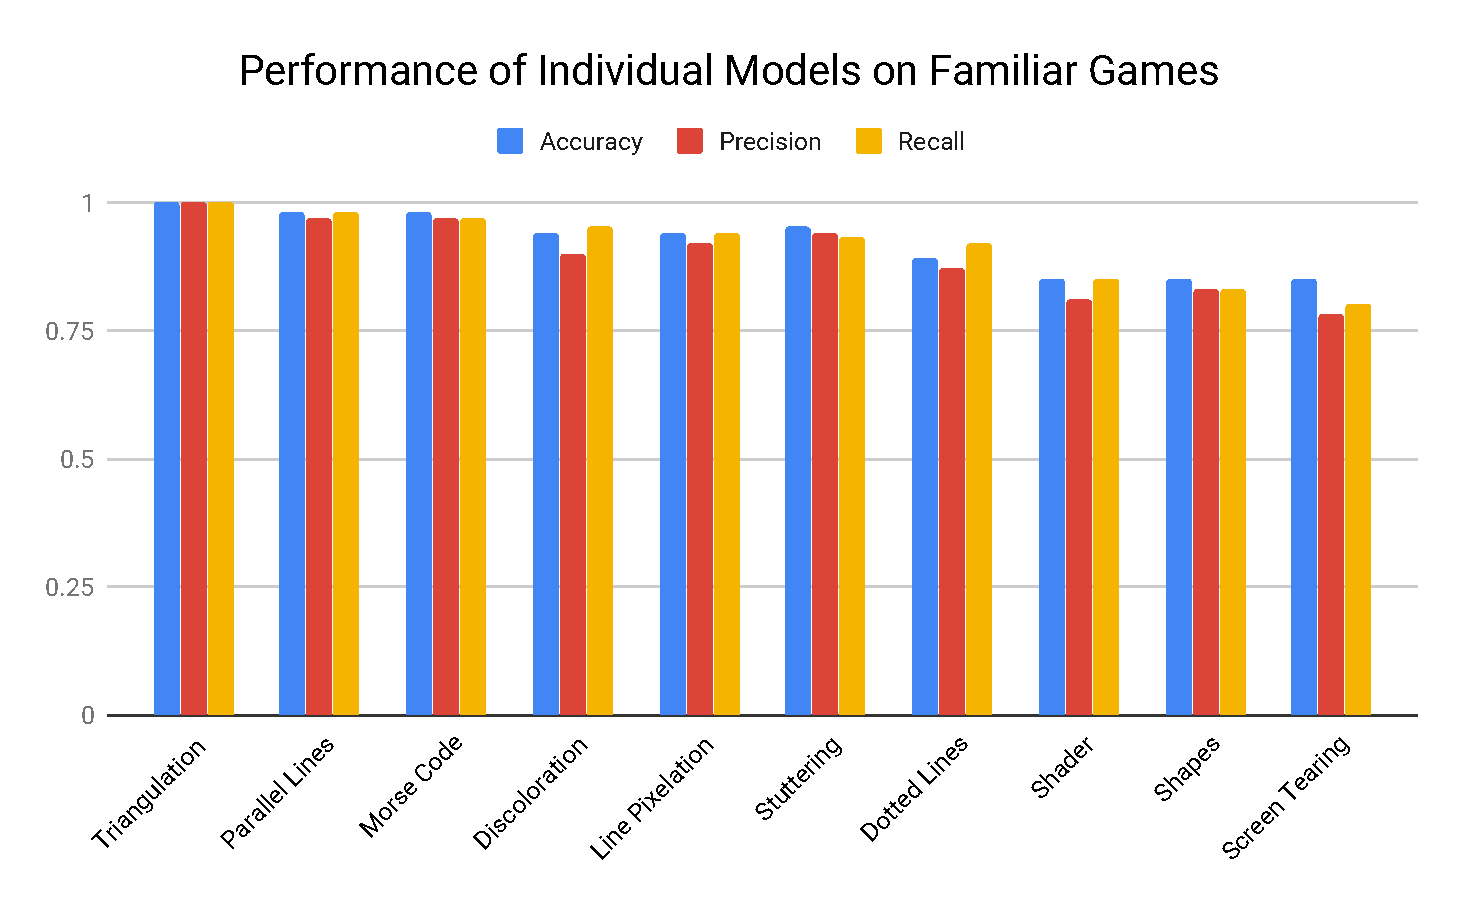
\includegraphics[scale=0.7]{images/stage1fig.pdf}
    \caption[Performance of models in training stage 1]{Performance of models in training stage 1. The models are tested on games they have seen before.}
    \label{fig:stage1}
\end{figure}


\begin{figure}
    \centering
    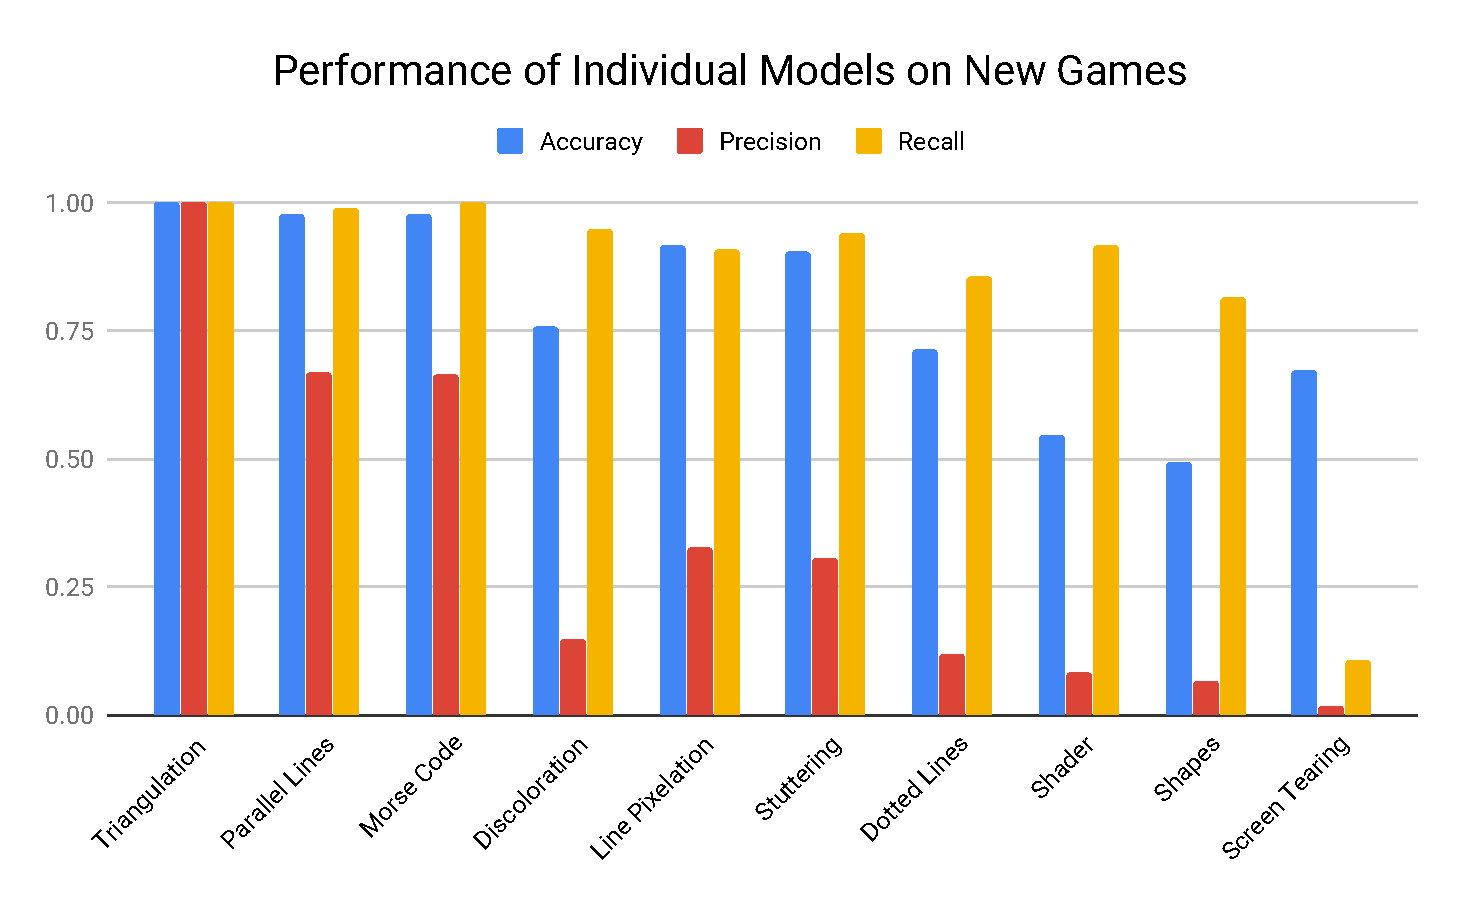
\includegraphics[scale=0.7]{images/stage2fig.pdf}
    \caption[Performance of models in training stage 2]{Performance of models in training stage 2. The models are tested on new games.}
    \label{fig:stage2}
\end{figure}


%\begin{table}
%    \centering
%    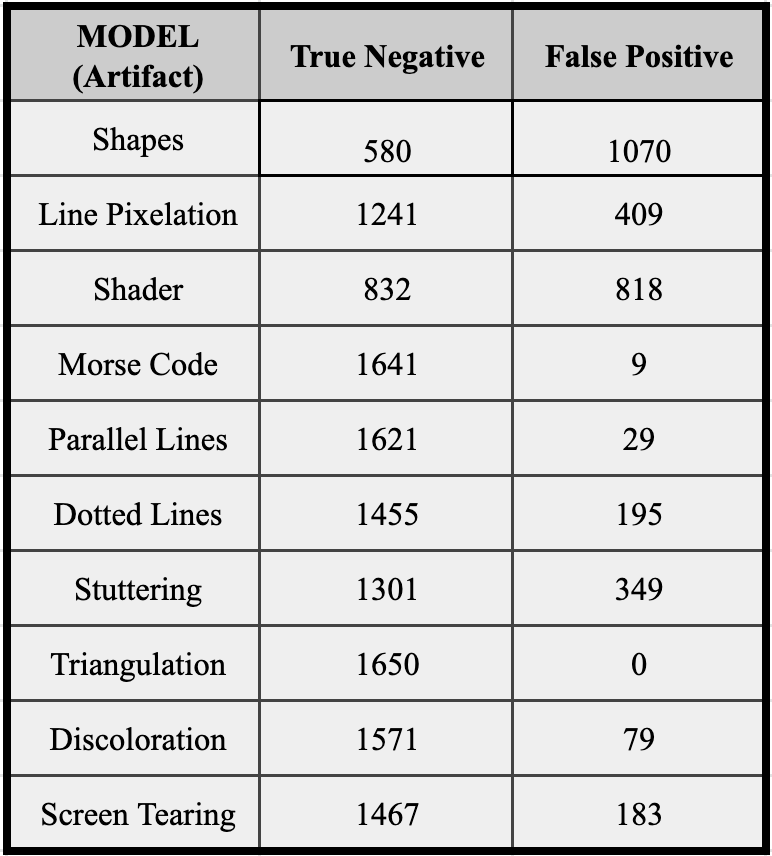
\includegraphics[scale=0.6]{tables/test_models.png}
%    \caption{Performance of models on the heldout test set.}
%    \label{tab:test_models}
%\end{table}

\begin{table}
\centering
\begin{tabular}{@{}lllll@{}}
\toprule
Model (Artifact) & True Negative & False Positive  \\ \midrule
Shapes & 580 & 1070\\
Line pixelation & 1241 & 409\\
Shader & 832 & 818\\
Morse code & 1641 & 9\\
Parallel lines & 1621 & 29\\
Dotted line & 1455 & 195\\
Stuttering & 1301 & 349\\
Triangulation & 1650 & 0\\
Discoloration & 1571 & 79\\
Screen tearing & 1467 & 183\\\bottomrule
\end{tabular}
\caption{Performance of models on the heldout test set.}
\label{tab:test_models}
\end{table}

%\begin{table}
%    \centering
%    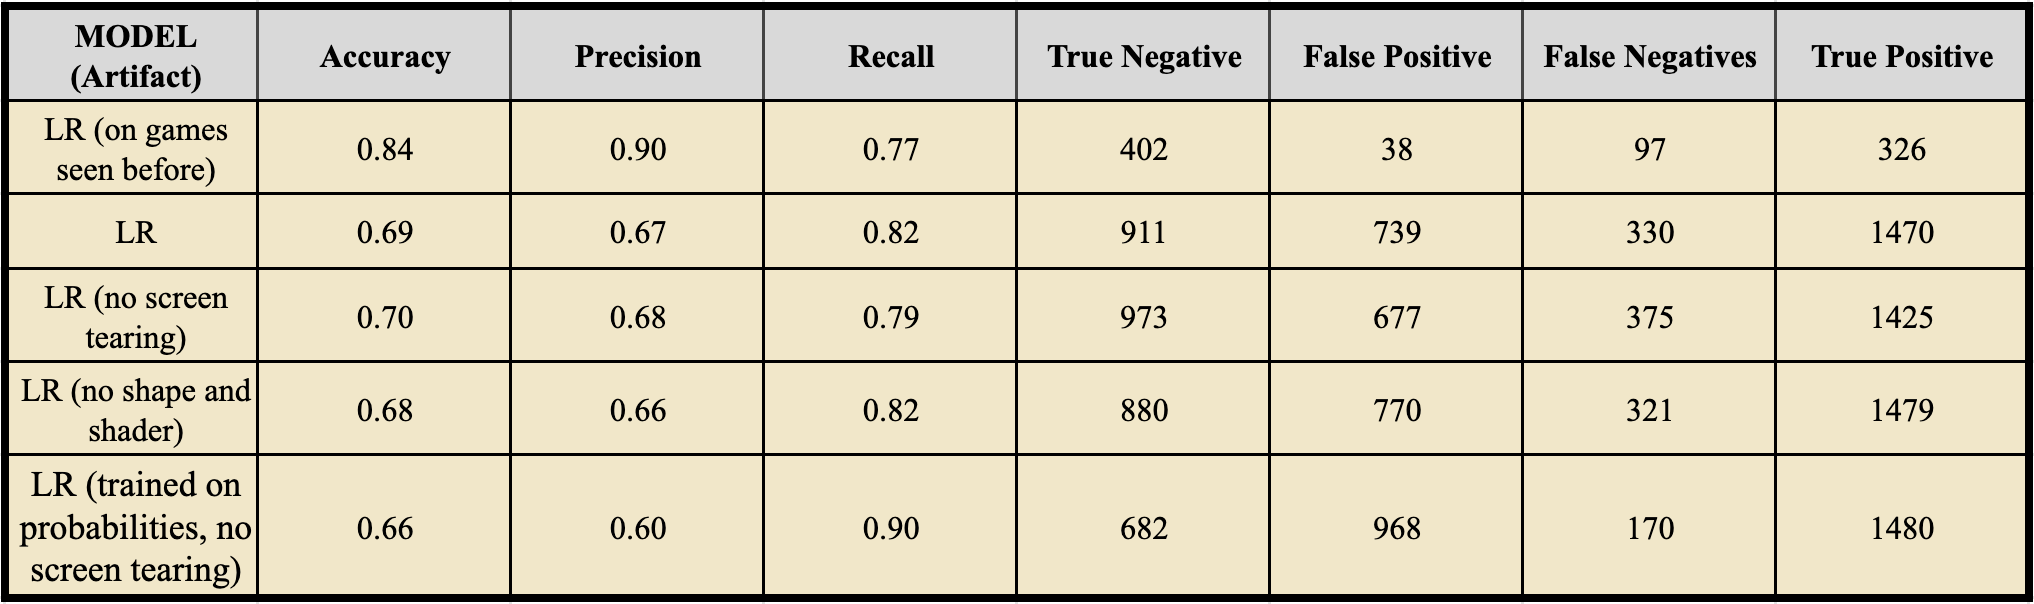
\includegraphics[scale=0.5]{tables/variation.png}
%    \caption{Performance of variations of LR.}
%    \label{tab:variation}
%\end{table}

\begin{table}
\centering
\begin{tabular}{@{}lllll@{}}
\toprule
Model & Accuracy & Precision & Recall  \\ \midrule
LR (full, seen games, binary) & 0.84 & 0.90 & 0.77\\
LR (full, unseen games, binary)& 0.69 & 0.67 & 0.82\\
LR (no screen tearing, unseen games, binary) & 0.70 & 0.68 & 0.79\\
LR (no shapes/shader, unseen games, binary) & 0.68 & 0.66 & 0.82\\
LR (full, unseen games, probability) & 0.66 & 0.60 &  0.90\\\bottomrule
\end{tabular}
\caption{Performance of variations of LR.}
\label{tab:variation}
\end{table}

\begin{figure}
    \centering
    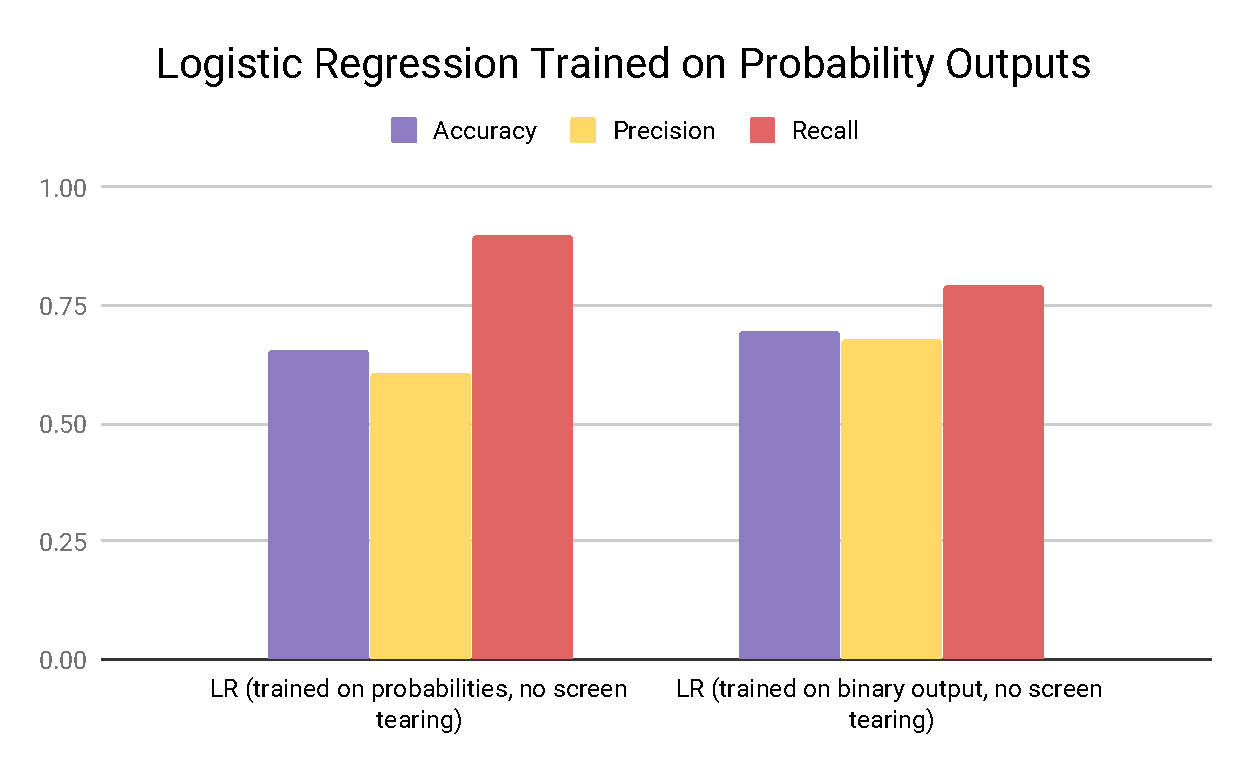
\includegraphics[scale=0.7]{images/probability.pdf}
    \caption[Performance of logistic regression on probability output]{The performance of the Logistic Regression trained on binary vs. probability output of the individual models.}
    \label{fig:probability}
\end{figure}




\section{Comparison to AMD's model}
AMD was able to run their model on our heldout test set (Data set C). In Figure \ref{fig:comparison} we can see that our models have similar accuracy, however, our model was able to achieve a higher recall score of 0.82 compared to AMD's score of 0.71.

\begin{figure}
    \centering
    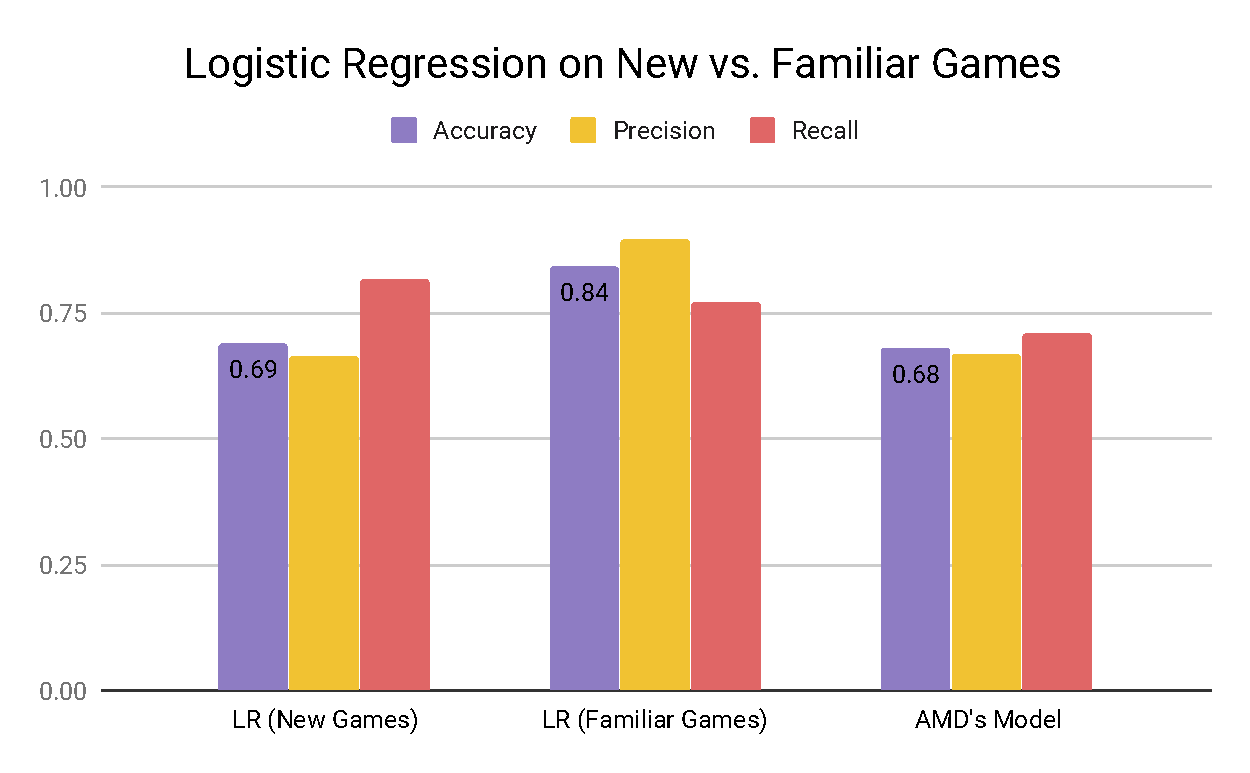
\includegraphics[scale=0.7]{images/comparison.pdf}
    \caption{Comparison of AMD's model and ours}
    \label{fig:comparison}
\end{figure}
\endinput
